\chapter{Hardwarové knihovny}
Hardwarové knihovny jsou nejnižší částí BlackBoxu.
Každá knihovna obsluhuje nějakou periferii a~slouží k~interakci s~ní.
Hardwarové knihovny jsou rozdělené\footnote{Pouze v~tomto textu, v~kódu toto rozdělení není.} do několika částí, které budou popsané dále v textu (každá odrážka představuje jednu knihovnu):

\begin{itemize}[noitemsep]
    \item Hlavní řídící modul
          \begin{itemize}[noitemsep]
              \item Real Time Clock
          \end{itemize}
    \item Uživatelské rozhraní
          \begin{itemize}[noitemsep]
              \item Touchpad
                    \begin{itemize}[noitemsep]
                        \item LDC
                    \end{itemize}
              \item LED kruh
          \end{itemize}
    \item Zámek
          \begin{itemize}[noitemsep]
              \item Zámek
              \item IR komunikace
          \end{itemize}
    \item Senzory prostředí
          \begin{itemize}[noitemsep]
              \item Senzory polohy
                    \begin{itemize}[noitemsep]
                        \item Magnetometr
                        \item Akcelerometr
                        \item Gyroskop
                    \end{itemize}
              \item Barometr
          \end{itemize}
\end{itemize}


\begin{figure}[h]
    \begin{small}
        \begin{center}
            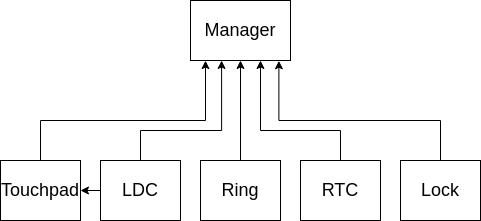
\includegraphics[width=0.95\textwidth]{img/manager.png}
        \end{center}
        \caption{Závislosti hardwarových knihoven}
        \label{fig:hLibs}
    \end{small}
\end{figure}

\section{Hlavní řídící modul}

Součástí hlavního modulu je samotný řídící čip ESP32 a RTC.

\subsection{RTC}\label{ss:rtc}

RTC slouží k~uchování času při šetření baterie tím, že umožňuje uspání zbytku BlackBoxu.
Stejně jako ostatní I$^2$C periferie\footnote{T.j. RTC, LDC, barometr, senzory polohy.} používá RTC virtuální dvojče tzn. že v~programu existuje kopie všech registrů, běžný uživatel pak pracuje pouze s~touto kopií, která se periodicky synchronizuje a~provádí přitom kontrolu nastavovaných hodnot.
Toto urychluje kontrolu nastavovacích registrů a~zároveň zjednodušuje potenciální tvorbu simulátoru.
Pokročilejší uživatelé mohou pracovat přímo s~jednotlivými registry a~dvojče používat pouze na rychlou kontrolu hodnot.

\section{Uživatelské rozhraní}

Uživatelské rozhraní je pro běžného uživatele asi nejužitečnější části knihovny, protože slouží právě k~interakci s~ním.

\subsection{Touchpad}

Třída Touchpad slouží jako most mezi uživatelem a~třídou LDC.
Je zodpovědná za přepočet surových dat z~LDC do souřadnic doteku a~jeho síly.

\begin{figure}[H]
    \begin{small}
        \begin{center}
            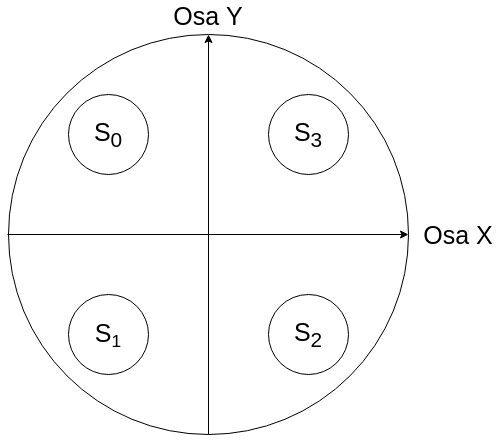
\includegraphics[width=0.95\textwidth]{img/Touchpad_calculation.png}
        \end{center}
        \caption{Výpočet pozice doteku}
        \label{fig:touchpad_calculation}
    \end{small}
\end{figure}

\begin{listedequation}[H]
    \begin{center}
        $X = -k_0S_0 -k_1S_1 +k_2S_2 +k_3S_3$\\
        $Y = +k_0S_0 -k_1S_1 -k_2S_2 +k_3S_3$\\
        $Tlak = \frac{k_0S_0 +k_1S_1 +k_2S_2 +k_3S_3}{4}$
    \end{center}
    \caption{Výpočet parametrů doteku}
    \label{eq:touchpad_calculation_X}
\end{listedequation}

\subsubsection{LDC}

Třída LDC se stará o~komunikaci s~čipem LDC1614.
Sama nedělá žádné výpočty, dělá pouze základní filtraci dat.
Jedná se o~I$^2$C senzor\footnote{Používá virtuální dvojče.~\autoref{ss:rtc}.}.

\subsection{LED kruh}

% ? Should I~write about 2.0?
LED kruh poskytuje kromě příjemného subscript operátoru pro přístup k~jednotlivým LED také možnost vykresloval celé obrazce (kružnice a~oblouky).
Umožňuje také nastavit maximální hodnotu displeje, všechny barvy jsou poté vyškálovány do tohoto rozsahu.
Za použití akcelerometru je také možné displej převracet v~závislosti na jeho natočení, jak je zvykem u~mobilních telefonů.

LED kruh je postaven na knihovně SmartLeds\cite{SmartLeds}.

\section{Zámek}

Tato sekce je důležitá především, pokud budete chtít používat Blackbox jako elektronický sejf.

\subsection{Lock}

Lock spravuje motor a~magnetický enkodér.
Ty dohromady tvoří zámek, který je schopen poznat, v~jakém stavu se nachází, bez nutnosti tuto informaci udržovat v~paměti.
Důležitý je fakt, že zámek je designovaný tak, aby se BlackBox dal vložit do protikusu, aniž by bylo nutné jej odemykat.

\subsection{IR komunikace}

IR komunikace je určená k~jednoduché komunikaci mezi BlackBox a~Chytrými zády\footnote{Protikus BlackBoxu s~vlastní elektronikou.}.


\section{Senzory prostředí}

\subsection{Senzory polohy}

Množství funkcionality poskytuje BlackBoxu možnost detekovat natočení v~9~osách. %todo tady toho asi dost chybí? 

\section{Příklady použití}

Hardwarové knihovny mají asi nejširší možnosti použití.
Dvěma z~nich mohou být i~herní a~výukové API.

Knihovny se nemusí používat pouze v~rámci desky BlackBox, ale také mimo ni jako samostatné knihovny.
Kupříkladu LED kruh se dá použít na řízení jakéhokoliv displeje, který má imitovat ručičkové ukazatele.
Touchpad může být sám o~sobě také velmi užitečný.
